\documentclass[10pt,twocolumn]{article}

\usepackage[margin=0.75in,columnsep=0.24in]{geometry}
\usepackage[T1]{fontenc}
\usepackage[utf8]{inputenc}
\usepackage{tgtermes}
\usepackage{microtype}
\usepackage{graphicx}
\usepackage{amsmath}
\usepackage{amssymb}
\usepackage{amsthm}
\usepackage{booktabs}
\usepackage{tabularx}
\usepackage{array}
\usepackage{hyperref}
\usepackage{caption}
\usepackage{float}

\setlength{\textfloatsep}{10pt plus 2pt minus 2pt}
\setlength{\floatsep}{8pt plus 2pt minus 2pt}
\setlength{\intextsep}{8pt plus 2pt minus 2pt}
\setlength{\dbltextfloatsep}{12pt plus 2pt minus 2pt}
\setlength{\abovecaptionskip}{4pt}
\setlength{\belowcaptionskip}{0pt}
\setlength{\parindent}{1em}
\setlength{\parskip}{0pt}
\renewcommand{\topfraction}{0.95}
\renewcommand{\bottomfraction}{0.9}
\renewcommand{\textfraction}{0.05}
\renewcommand{\floatpagefraction}{0.85}
\renewcommand{\dbltopfraction}{0.95}
\renewcommand{\dblfloatpagefraction}{0.85}

\hypersetup{
  colorlinks=true,
  linkcolor=[rgb]{0.05,0.20,0.55},
  citecolor=[rgb]{0.05,0.20,0.55},
  urlcolor=[rgb]{0.05,0.20,0.55}
}

\captionsetup{font=small,labelfont=bf}

\newcommand{\fanda}{\textsc{FAnDa}}
\newcommand{\dola}{\textsc{DoLa}}
\newcommand{\truthfulqa}{\textsc{TruthfulQA}}
\newtheorem{proposition}{Proposition}

\makeatletter
\renewcommand{\maketitle}{%
  \begin{center}
    {\LARGE\bfseries \@title \par}
    \vspace{0.4em}
  \end{center}
  \vspace{-0.6em}
}
\renewcommand\section{\@startsection{section}{1}{\z@}%
  {-1.8ex \@plus -0.2ex \@minus -0.2ex}%
  {0.8ex \@plus 0.2ex}%
  {\large\bfseries}}
\renewcommand\subsection{\@startsection{subsection}{2}{\z@}%
  {-1.3ex \@plus -0.2ex \@minus -0.2ex}%
  {0.5ex \@plus 0.2ex}%
  {\normalsize\bfseries}}
\makeatother

\title{\fanda: Frozen Anchor Contrastive \dola\ for More Stable Truthful Decoding}
\author{}
\date{}

\begin{document}

\twocolumn[
\begin{@twocolumnfalse}
\maketitle
\begin{abstract}
We revisit \dola\ as a truthfulness-oriented decoding method and ask whether two design choices are actually necessary: relative-top filtering and per-token reselection of the shallow contrast layer. We propose \fanda\ (Frozen Anchor Contrastive \dola), a simpler variant that removes the relative-top filter, contrasts in raw-logit space, and freezes a single shallow anchor for the whole generation. On a matched \truthfulqa\ multiple-choice comparison with \texttt{Qwen/Qwen2.5-3B-Instruct}, \fanda\ improves over official \dola\ from $(\mathrm{mc1}, \mathrm{mc2}, \mathrm{mc3}) = (0.28, 0.528, 0.273)$ to $(0.40, 0.576, 0.351)$. Two ablations explain where this gain comes from: a matched $2 \times 2$ study shows that removing the relative-top filter is the dominant effect, while a persistence study shows that more stable anchor schedules outperform token-local reselection and sharply reduce shallow-layer switching. Open-ended evaluation is more mixed: update1 achieves the highest mean manual score, but the frozen-anchor variant remains competitive and wins a targeted long-generation stress test by a small margin. The evidence suggests that stable contrast references are a strong design bias for factual short-answer decoding, while broader open-ended superiority remains unproven.
\end{abstract}
\vspace{1.0em}
\end{@twocolumnfalse}
]

\section{Introduction}
Large language models often know correct facts while still producing misleading continuations. This has made inference-time decoding a practical target for truthfulness improvements, especially when retraining is expensive or unavailable. \dola\ is a strong representative of this line of work: it contrasts later and earlier transformer layers to produce more factual outputs \cite{dola}. The question in this paper is not whether contrastive decoding helps in general, but whether the specific \dola\ configuration is more complicated than it needs to be.

We focus on two design choices in official \dola. First, it applies a relative-top filter before final token selection. Second, it can change the shallow comparison layer from token to token. Both choices are plausible, but both can also create unwanted behavior: the filter may prune away useful candidates too early, and token-wise reselection may make the correction signal itself unstable.

This motivates \fanda, short for \emph{Frozen Anchor Contrastive \dola}. \fanda\ keeps the contrastive intuition of \dola, but removes the relative-top filter, uses raw-logit contrast, and freezes a single shallow anchor for the entire generation. The resulting decoder is simpler, easier to interpret, and more stable by construction.

The paper makes three claims. First, \fanda\ is a stronger matched multiple-choice decoder than official \dola\ in the setup studied here. Second, that gain comes primarily from removing the filter and stabilizing the anchor, not from introducing a more elaborate token-level control rule. Third, the open-ended story is mixed: frozen anchoring is competitive and often more robust, but not uniformly best on average. That final nuance matters, because it keeps the conclusions honest.

\section{Method}
\dola\ can be viewed as contrasting a mature layer with a shallower layer to obtain a corrected next-token preference. Let $z_t^{(L)}$ denote the final-layer vocabulary logits at generation step $t$. In the \dola-style formulation studied here, the shallow reference may vary with time:
\[
s_t^{\text{\dola}} \propto z_t^{(L)} - z_t^{(a_t)},
\]
where $a_t$ is a selected shallow layer.

\fanda\ keeps the same contrastive template but fixes the shallow anchor once at the beginning of generation:
\[
s_t^{\text{\fanda}} \propto z_t^{(L)} - z_t^{(a)},
\]
where $a$ is constant over the entire answer. In the implementation studied here, \fanda\ also removes the relative-top filter and performs contrast directly in raw-logit space.

The design intuition is simple. Factuality is judged at the sequence level, but decoding happens token by token. If the shallow contrast layer changes every step, then the decoder is also changing the lens through which it judges each continuation. Some observed token differences may then reflect decoder jitter rather than a better answer. A frozen anchor keeps the correction signal consistent across the whole sequence and should therefore reduce one source of instability. This intuition is consistent with broader sequence-modeling arguments about persistent state and cross-position continuity \cite{attention,qwen25}.

\paragraph{A stability interpretation.}
Let $g_t^\star$ denote the step-local contrast score that reselects the shallow layer at token $t$, and let $g_t^{(k)}$ denote the schedule-$k$ score that reuses the most recent anchor for $k$ steps. Then
\[
g_t^{(k)} = g_t^\star + e_t^{(k)},
\]
where $e_t^{(k)}$ is exactly the stale-anchor mismatch induced by persistence.

\begin{proposition}[Informal token and ranking stability]
Let $m_t$ be the oracle top-token margin under $g_t^\star$. If $2\|e_t^{(k)}\|_\infty < m_t$, then the schedule-$k$ decoder chooses the same next token as the step-local oracle. Under teacher-forced multiple-choice scoring, candidate rankings are likewise preserved whenever the cumulative stale-anchor perturbation stays below the oracle sequence margin.
\end{proposition}

This proposition gives the main paper-safe takeaway from the derivation: persistence affects decoding only through shallow-anchor mismatch, so moderate anchor reuse can suppress selector jitter without yet changing the intended ranking. A simple perturbation model $R(k) \lesssim A/k + Bk$ further explains why an interior schedule such as \texttt{update4} can outperform both \texttt{update1} and a fully frozen anchor: frequent refreshes pay a jitter cost, while very long reuse pays a staleness cost. Figure~\ref{fig:fanda-algorithm} summarizes this sequence-level view of the decoder. The argument supports a stability interpretation of \fanda, not a universal proof of open-ended factuality.

\begin{figure*}[t]
    \centering
    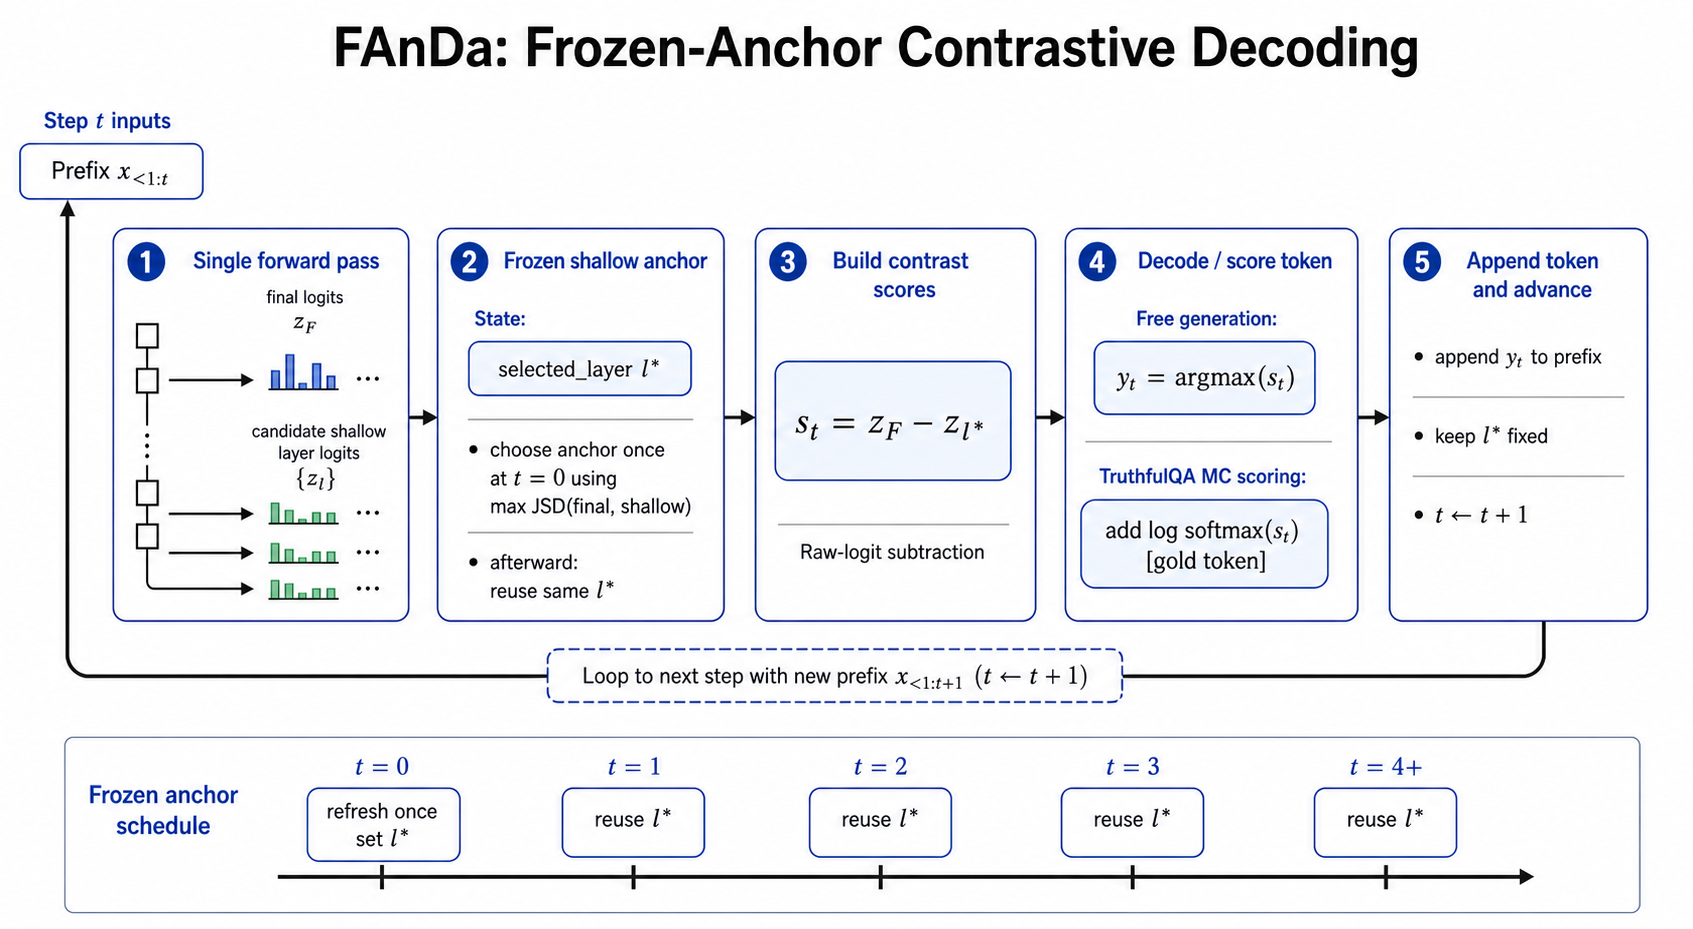
\includegraphics[width=0.9\textwidth]{assets/fanda_algorithm_diagram.png}
    \caption{Conceptual workflow of \fanda. The decoder chooses a shallow anchor once, keeps that anchor fixed across subsequent decoding steps, and applies the same contrast reference throughout the answer. Promoting the figure to a wide layout highlights the method as a sequence-level stabilization rule rather than a token-local control heuristic.}
    \label{fig:fanda-algorithm}
\end{figure*}

\section{Experimental Setup}
All experiments use \texttt{Qwen/Qwen2.5-3B-Instruct}. The main benchmark is the multiple-choice subset of \truthfulqa\ \cite{truthfulqa}, with a matched 50-question subset used for the direct decoder comparison and the key ablations. We report $\mathrm{mc1}$, $\mathrm{mc2}$, and $\mathrm{mc3}$ for truthfulness, and decoding latency for efficiency.

To test long-form behavior, we additionally run an open-ended evaluation in which 250 answers are scored on a 0/1/2 rubric: 0 for wrong or hallucinated, 1 for mixed or noisy, and 2 for broadly correct. The source material reports these manual judgments using GPT-5.4 over full generated answers. We also use a targeted long-generation subset of 8 prompts to probe robustness more directly.

\section{Main Result: \fanda\ Improves Over \dola}
The clearest paper-level result is the matched decoder comparison in Table~\ref{tab:core-results}. On the 50-question \truthfulqa\ subset, \fanda\ improves over official \dola\ on all three multiple-choice factuality metrics:
\[
(\mathrm{mc1}, \mathrm{mc2}, \mathrm{mc3})_{\text{\dola}} = (0.28, 0.528, 0.273)
\]
\[
(\mathrm{mc1}, \mathrm{mc2}, \mathrm{mc3})_{\text{\fanda}} = (0.40, 0.576, 0.351).
\]

These gains matter because they are achieved with a simpler decoder rather than a more complex one. \fanda\ does not add a learned controller, extra training, or a more aggressive token-level arbitration scheme. Its improvements come from removing a filter and enforcing anchor stability.

\begin{table}[!t]
    \centering
    \footnotesize
    \setlength{\tabcolsep}{3pt}
    \begin{tabular}{lcccc}
        \toprule
        Decoder & MC1 & MC2 & MC3 & Step ms \\
        \midrule
        Greedy & 0.340 & 0.531 & 0.307 & \textbf{39.7} \\
        Top-$k$ & 0.040 & 0.222 & 0.040 & 40.9 \\
        Top-$p$ & 0.000 & -- & 0.000 & 41.3 \\
        \dola & 0.280 & 0.528 & 0.273 & 79.1 \\
        PAnDa & 0.340 & \textbf{0.561} & 0.314 & 180.7 \\
        \fanda & \textbf{0.400} & 0.560 & \textbf{0.364} & 85.3 \\
        \bottomrule
    \end{tabular}
    \caption{Matched core decoder comparison on the 50-question \truthfulqa\ subset. \fanda\ provides the strongest overall factuality profile among the simple contrastive decoders while remaining much cheaper than PAnDa.}
    \label{tab:core-results}
\end{table}

\section{Why \fanda\ Works}
\subsection{The Relative-Top Filter Is the Main Liability}
The first ablation isolates two candidate explanations for \dola's weakness: score space and filtering. We run a matched $2 \times 2$ factorial over raw logits versus log-probabilities and relative-top filtering on versus off, while holding the rest of the decoder fixed.

\begin{table}[!t]
    \centering
    \small
    \begin{tabular}{lccc}
        \toprule
        Variant & MC1 & MC2 & MC3 \\
        \midrule
        logprob + filter & 0.280 & 0.528 & 0.273 \\
        logprob, no filter & 0.380 & 0.527 & 0.329 \\
        raw-logit + filter & 0.300 & 0.520 & 0.300 \\
        raw-logit, no filter & 0.380 & 0.527 & 0.329 \\
        \bottomrule
    \end{tabular}
    \caption{Matched $2 \times 2$ filter ablation. Removing the relative-top filter is the dominant effect; switching from log-probability to raw-logit contrast has only a small and mixed impact.}
    \label{tab:filter-ablation}
\end{table}

Table~\ref{tab:filter-ablation} makes the central pattern explicit: the no-filter variants are the strongest ones, especially on $\mathrm{mc1}$ and $\mathrm{mc3}$. By contrast, changing score space from log-probability to raw-logit produces only a small and mixed effect. This strongly suggests that the main gain comes from preserving candidate tokens until the final contrastive decision rather than from a change in numerical representation.

\subsection{Stable Anchors Beat Token-Local Reselection}
After removing the filter, the next question is whether the shallow anchor should still be reselected at every token. To test this, we compare matched variants that differ only in refresh schedule: \texttt{update1}, \texttt{update2}, \texttt{update4}, and \texttt{frozen}.

\begin{table}[!t]
    \centering
    \small
    \begin{tabular}{lcccc}
        \toprule
        Schedule & MC1 & MC2 & MC3 & Switch rate \\
        \midrule
        update1 & 0.340 & 0.534 & 0.294 & 0.692 \\
        update2 & 0.380 & 0.527 & 0.331 & 0.323 \\
        update4 & 0.400 & 0.576 & 0.351 & 0.135 \\
        frozen & 0.400 & 0.560 & 0.364 & 0.000 \\
        \bottomrule
    \end{tabular}
    \caption{Anchor persistence ablation. More persistent schedules improve factuality while sharply reducing shallow-layer switching.}
    \label{tab:persistence}
\end{table}

Table~\ref{tab:persistence} shows the same tradeoff in a more paper-like form. Token-local \texttt{update1} is never the best setting, while the more persistent schedules dominate the factuality metrics and cut switching dramatically. The most attractive balance is \texttt{update4}, which matches the best $\mathrm{mc1}$, gives the strongest $\mathrm{mc2}$, and reduces switch rate by about 80\% relative to \texttt{update1}. The fully frozen anchor pushes stability even further and produces the best $\mathrm{mc3}$.

\section{Open-Ended Evaluation}
The short-answer multiple-choice evidence clearly favors persistent anchors, but the open-ended story is more nuanced. On the 250-answer manual evaluation, \texttt{update1} achieves the best mean score, while \texttt{frozen} remains a close second.

\begin{table}[!b]
    \centering
    \small
    \begin{tabular}{lccc}
        \toprule
        Decoder & Mean score & Score-2 rate & Score-0 rate \\
        \midrule
        update1 & 0.62 & 0.16 & 0.54 \\
        update2 & 0.52 & 0.10 & 0.58 \\
        update4 & 0.38 & 0.06 & 0.68 \\
        update8 & 0.44 & 0.08 & 0.64 \\
        frozen & 0.56 & 0.16 & 0.60 \\
        \bottomrule
    \end{tabular}
    \caption{Open-ended manual evaluation over 250 answers. Update1 has the strongest mean score, while frozen remains the closest competitor and matches the best score-2 rate.}
    \label{tab:openended}
\end{table}

Table~\ref{tab:openended} prevents the strongest possible claim: frozen anchoring is not uniformly superior on long-form generation. In the reported results, \texttt{update1} reaches the best mean manual score at 0.62, while \texttt{frozen} reaches 0.56 and matches the best score-2 rate. This is still close enough to justify a more targeted robustness probe rather than dismissing the frozen-anchor idea.

That probe gives the final qualitative result of the paper. On an 8-question long-generation stress test selected from the broader manual review, \texttt{frozen} wins 4 prompts, \texttt{update1} wins 3, and 1 is effectively tied. The broader source analysis also suggests a plausible reason: higher-scoring open-ended answers tend to be shorter, while worse answers more often drift into repetition, unsupported detail, or garbling. The frozen-anchor mechanism may therefore be especially helpful when the main challenge is late-generation drift rather than average open-ended score.

\section{Discussion}
The main lesson from these experiments is that better factual decoding does not necessarily require more reactive token-level control. In the setup studied here, \fanda\ improves over \dola\ by doing less: it keeps more candidates alive and keeps the contrast lens fixed.

This matters conceptually because it shifts the design bias for truthful decoding. A natural instinct is to make the decoder increasingly adaptive, switching layers or rules whenever the local token context changes. The evidence here points in a different direction. When the decoder itself keeps changing its reference frame, some of what looks like smarter control may instead be instability. A fixed anchor is not globally optimal, but it is a strong regularizer against that failure mode.

\section{Limitations}
The evidence is promising but narrow. First, the key multiple-choice comparisons use a 50-question \truthfulqa\ subset, which is enough to reveal clear directional patterns but not enough to settle small statistical differences. Second, all experiments use a single model family, \texttt{Qwen/Qwen2.5-3B-Instruct}. Third, the paper combines benchmark scoring with manual open-ended judgment, and those two regimes capture different notions of quality. Finally, the targeted long-generation comparison is intentionally selected from the larger open-ended pool, so it should be read as a stress test rather than an unbiased sample.

These limitations narrow the claim but do not erase it. The paper supports \fanda\ as a better matched replacement for the official \dola\ setup studied here; it does not show that frozen anchors are universally optimal for all models, prompts, or long-form tasks.

\section{Conclusion}
\fanda\ is a simple revision of \dola\ with a clear empirical story. Its gains over official \dola\ come primarily from two changes: removing the relative-top filter and stabilizing the shallow contrast anchor. These changes improve multiple-choice factuality, reduce anchor-switching noise, and remain competitive under open-ended evaluation. The strongest overall conclusion is therefore modest but useful: for truthfulness-oriented decoding, a stable contrast reference is a powerful baseline and may be preferable to more aggressively adaptive token-level control.

\begin{thebibliography}{9}\small
\setlength{\itemsep}{0.35em}

\bibitem{attention}
Ashish Vaswani, Noam Shazeer, Niki Parmar, Jakob Uszkoreit, Llion Jones, Aidan N. Gomez, Lukasz Kaiser, and Illia Polosukhin.
\newblock Attention Is All You Need.
\newblock In \emph{Advances in Neural Information Processing Systems}, 2017.
\newblock \url{https://arxiv.org/abs/1706.03762}

\bibitem{truthfulqa}
Stephanie Lin, Jacob Hilton, and Owain Evans.
\newblock TruthfulQA: Measuring How Models Mimic Human Falsehoods.
\newblock In \emph{Proceedings of ACL}, 2022.
\newblock \url{https://arxiv.org/abs/2109.07958}

\bibitem{dola}
Yung-Sung Chuang, Yujia Xie, Hongyin Luo, Yoon Kim, James Glass, and Pengcheng He.
\newblock DoLa: Decoding by Contrasting Layers Improves Factuality in Large Language Models.
\newblock In \emph{Proceedings of ICLR}, 2024.
\newblock \url{https://arxiv.org/abs/2309.03883}

\bibitem{qwen25}
An Yang, Baosong Yang, Beichen Zhang, Binyuan Hui, Bo Zheng, Bowen Yu, Chengyuan Li, Dayiheng Liu, Fei Huang, and collaborators.
\newblock Qwen2.5 Technical Report.
\newblock arXiv preprint arXiv:2412.15115, 2025.
\newblock \url{https://arxiv.org/abs/2412.15115}

\end{thebibliography}

\end{document}
